\title{COM S 352 Homework 1}
\author{Alec Meyer}

\date{\today}

\documentclass[11pt]{article}
\usepackage{changepage}
\usepackage{graphicx}
\usepackage{amsmath}
\graphicspath{ {./images/} }
\newcommand\tab[1][1cm]{\hspace*{#1}}
\usepackage{amssymb}


\begin{document}
\maketitle


\section*{Question 1}
Interrupts are used to inform a program or proccess
of an external proccess, typically a physical 
device controller telling the CPU that there has 
been an I/O operation. A Trap, However, is an interrupt 
triggered by software (i.e. exceptions, requests
from other programs). Traps can be generated 
intentionally such as an exception being thrown when
trying to access invalid memory or invalid 
arithmetic.

\section*{Question 2}
The two modes of a CPU are User mode and Kernel mode.
The system privlleges are increased when Kernal mode
is in use because Kernal mode will allow more control
over the system. Only Kernal mode can run privlleged
instructions, such as clearing memory and accessing
I/O devices. This dual operation will help protect
the user and the system from programs not laucnhing 
correctly and/or being malicious. The reason to 
distinguish the two is to know where interrupts
should be used. The system will produce interrupts 
in user mode then switch to Kernel mode.

\section*{Question 3}
\textbf{Privlleged Instructions:}\\
Clearing memory\\
Turning off Interrupts\\
Putting the CPU in Kernel mode\\
Accessing I/O device\\
Setting value of timer

\section*{Question 4}
1,000 CPU cycles per 1 $\mu$s\\
20 bytes every 10 $\mu$s = 20 bytes every 10,000 cycles\\\\
10,000 cycles sending\\
100 cycles transfering to memory\\
10,000 + 100 cycles = 10,100 total cycles\\\\
\( \frac{\text{100 Transfering Cycles}}
{\text{10,100 Total Cycles}} \) = $0.99$\% $\approx 1$\%\\\\
about 1\% of the CPU clock cycles are used to 
transfer data from the controller to main memory.


\section*{Question 5}
\begin{enumerate}
    \item \textbf{Program 1}\\
    50ms computation\\
    100ms I/O\\
    device 1
    \item \textbf{Program 2}\\
    20ms computation\\
    50ms I/O\\
    device 1
    \item \textbf{Program 3}\\
    50ms computation\\
    100ms I/O\\
    device 2
\end{enumerate}
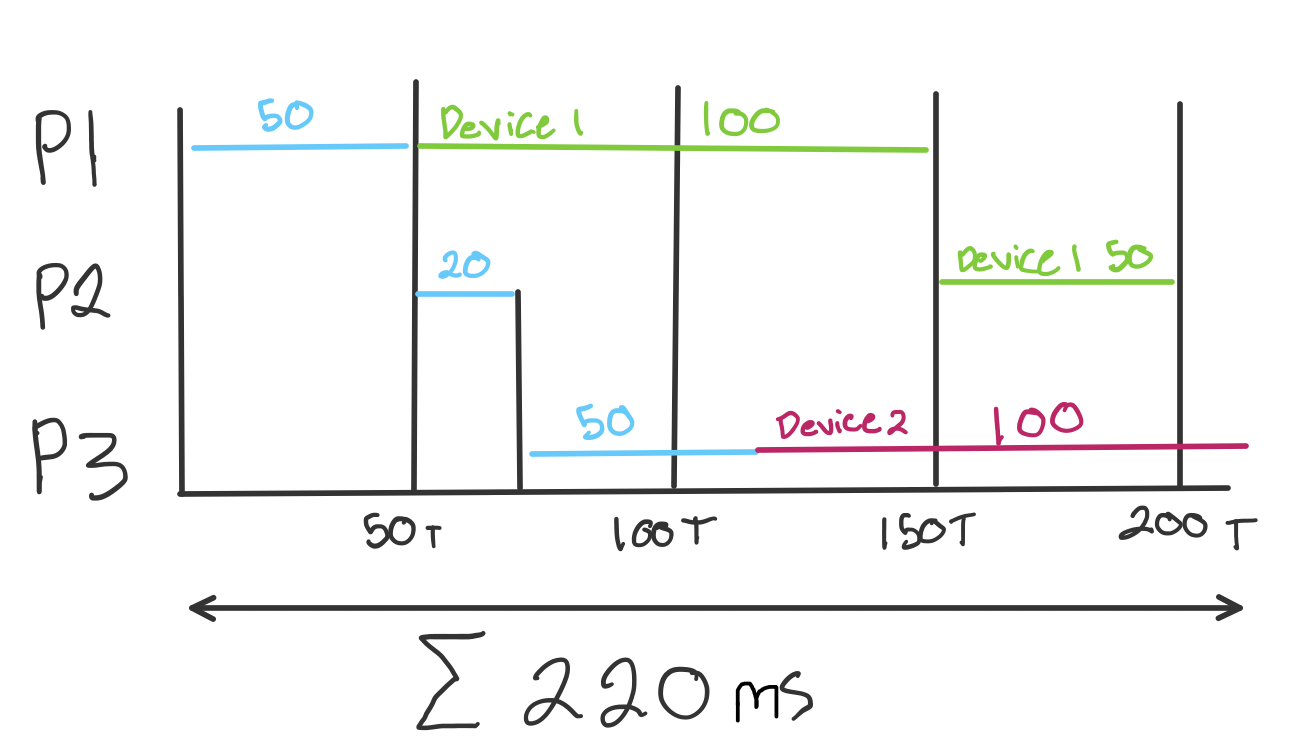
\includegraphics[scale=0.3]{diagram}

\section*{Question 6}
A DMA controller does not require the CPU to 
interviene while writing data. This allows the 
CPU to preform other tasks while data is being
transfered. interrupt driven I/O requires the 
CPU's attention and also only writes one byte at
a time.

\section*{Question 7}
\begin{enumerate}
\item \textbf{Parameters in Registers}\\
Simplest method, can only have as many 
parameters as available registers. Most 
operating systems do not use this method as 
it only allows a few parameters of a certain
length at a time.

\item \textbf{Parameters in Block Memory}\\
If there are more parameters than registers
the extra parameters will be saved to a block or 
table of memory. Then the address is used as the 
parameter.

\item \textbf{Parameters in Stacks}\\
Similar to the block memory aproach the
stack approach is when you push parameters on
a stack and pop them when they are to be used.

\end{enumerate}
\end{document}

